\documentclass{article}
\usepackage{graphicx} % Required for inserting images
\usepackage[ngerman]{babel}
\usepackage{enumitem}
\usepackage{float}
\usepackage{chngcntr}
\usepackage{glossaries}
\usepackage{tabularx}
\usepackage{hyperref}
\usepackage{titletoc}
\usepackage{titlesec}
\usepackage{csquotes}
\usepackage{pgf-pie}   
\usepackage{glossaries-extra}
\counterwithin{figure}{section}
\counterwithin{table}{section}
\setlength\parindent{0pt}

\titleformat{\paragraph}[runin]{\large\bfseries}{\theparagraph}{}{}

\newcommand{\classref}[1]{\texttt{#1}}
\newcommand{\guibutton}[1]{\fbox{\texttt{#1}}}

\makeglossaries

\newacronym{Ableitung}{Ableitung}{Attributsableitung}

\newglossaryentry{Alternative}
{
    name=Alternative,
    description={Ein alternatives Verkehrsmittel im Modell. Besteht aus einem Namen und einer Nutzenfunktion, die im Allgemeinen Referenzen auf Attribute oder Attributsableitungen besitzt}
}

\newglossaryentry{Attributsableitung}
{
    name=Attributsableitung,
    description={Besteht aus einem Namen und einem Ausdruck aus existierenden Spalten der Tabelle oder anderen Attributsableitungen}
}

\newglossaryentry{biogeme}
{
    name=biogeme,
    description={Ein Python-Modul, welches Methoden zur Berechnug von Discrete Choice Modelle enthält}
}

\newacronym{CSV}{CSV}{Comma-separated values}

\newglossaryentry{Discrete Choice Model}
{
    name=Discrete Choice Modell,
    description={Statistisches Modell zur Analyse von Entscheidungsverhalten zwischen verschiedener Alternativen}
}

\newglossaryentry{Diskretes Wahlmodell}
{
    name=Diskretes Wahlmodell,
    description={Deutsche Übersetzung von \emph{Discrete Choice Model}}
}

\newglossaryentry{Erhebungsdaten}
{
    name=Erhebungsdaten,
    description={Vom Nutzer importierbare Daten in tabellarischer Form. Bilden die Grundlage für das Erstellen von Attributsableitungen und Alternativen, sowie für die Berechnung der Parameterschätzung}
}

\newacronym{GANTT}{GANTT}{Diagramm für Projektmanagement, das die zeitliche Abfolge von Aktivitäten grafisch in Form von Balken auf einer Zeitachse darstellt}

\newacronym{GUI}{GUI}{Graphical User Interface / Grafische Benutzeroberfläche}

\newglossaryentry{immutable}
{
    name=\textit{\flqq{}immutable\frqq},
    description={Eigenschaft einer Klasse, bei der die eigenen Klassenattribute unveränderlich sind. Verändert werden können dennoch Objekte, auf die durch eine Klasse referenziert wird, sofern diese nicht \emph{immutable} sind}
}

\newglossaryentry{Invalide Alternative}
{
    name=Invalide Alternative,
    description={Eine Alternative, dessen Name bereits vorkommt, dessen Nutzenfunktion syntaktisch inkorrekt ist oder die eine Referenz auf ein nicht-existierendes Attribut hat}
}

\newglossaryentry{Invalide Attributsableitung}
{
    name=Invalide Attributsableitung,
    description={Eine Attributsableitung, dessen Name bereits vorkommt, die syntaktisch inkorrekt ist oder die eine Referenz auf ein nicht-existierendes Attribut hat}
}

\newacronym{JSON}{JSON}{JavaScript Object Notation}

\newacronym{MVC}{MVC}{Model-View-Controller}

\newglossaryentry{pandas}
{
    name=pandas,
    description={Ein Python-Modul, welches sich zum Einlesen und zur Datenhaltung von CSV-Dateien eignet}
}

\newglossaryentry{Projektdatei}
{
    name=Projektdatei,
    description={Enthält potentiell eine CSV-Datei, sowie eventuell Attributsableitungen, Alternativen und vorherige Ergebnisse}
}

\newglossaryentry{PyQt}
{
    name=PyQt,
    description={Python Plug-in zur Erstellung von GUIs}
}

\newacronym{Rohdaten}{Rohdaten}{Erhebungsdaten}

\newglossaryentry{Unit-Test}
{
    name=Unit-Test,
    description={Eine Schnittstelle zum automatisiert testen von Quellcode}
}

\newglossaryentry{Valide Alternative}
{
    name=Valide Alternative,
    description={Eine Alternative, dessen Name eindeutig ist, dessen Nutzenfunktion syntaktisch korrekt ist und dessen Referenzen auf Attribute alle existieren}
}

\newglossaryentry{Valide Attributsableitung}
{
    name=Valide Attributsableitung,
    description={Eine Attributsableitung, dessen Name eindeutig ist, die syntaktisch korrekt ist und dessen Referenzen auf Attribute alle existieren}
}


\title{Implementierungsbericht \\ \large Discrete Choice Model Builder}
\author{Kevin Boehnke \\ \texttt{uxpkw@student.kit.edu}
\and Floriane Bresser \\ \texttt{uspvq@student.kit.edu}
\and Damian Reich \\ \texttt{uqppn@student.kit.edu}
\and Alissa Saleh \\ \texttt{unmbc@student.kit.edu}
\and Michael Schur \\ \texttt{ufkmz@student.kit.edu}}
\date{21. Juli 2023}

\begin{document}
\maketitle
\thispagestyle{empty}
\newpage
\startcontents[maintableofcontents]
\printcontents[maintableofcontents]{}{1}[2]{\section*{Inhaltsverzeichnis}}
\thispagestyle{empty}
\newpage
\pagenumbering{arabic}

\section{Einleitung}
%Einleitung mit Anschluss auf Pflichtenheft und Entwurf

Die Implementierungsphase markiert einen entscheidenden Abschnitt in der Entwicklung unseres Discrete Choice Model Builders. In dieser Phase findet der Übergang von der theoretischen Planung zur praktischen Umsetzung statt. Es ist der Moment, in dem das Projekt zum Leben erweckt wird und die in der Entwurfsphase erarbeiteten Konzepte, Modelle und Spezifikationen konkret umgesetzt werden, um das geplante System in die Realität zu überführen.

Ein detailliertes Pflichtenheft, das in den vorangegangenen Phasen erstellt wurde, dient dabei als Leitfaden und Referenz, um sicherzustellen, dass die implementierte Lösung alle Anforderungen und Funktionalitäten erfüllt. Hierbei können auch kleinere Anpassungen am Pflichtenheft notwendig werden, um etwaige Unklarheiten oder neue Erkenntnisse zu berücksichtigen. \\

In der Implementierungsphase werden die notwendigen Funktionen und Module erstellt und miteinander verknüpft, um ein reibungslos funktionierendes Gesamtsystem zu schaffen. Eine klare Kommunikation und ein effektives Projektmanagement sind dabei entscheidend, um den Implementierungsprozess erfolgreich abzuschließen. Am Ende der Implementierungsphase sollte der Baukasten zur Discrete Choice Modellierung funktionsfähig sein und die in der Entwurfsphase festgelegten Ziele erreichen. Der Fokus liegt dabei auf Fehlertoleranz, die Bedienbarkeit, die Änderbarkeit.

Eine gründliche Testphase wird folgen, um sicherzustellen, dass das System zuverlässig und fehlerfrei arbeitet, bevor es schließlich den Benutzern zur Verfügung gestellt wird. \\

Zusammenfassend kann man sagen, dass die Implementierungsphase eine Phase der Umsetzung und Realisierung ist, in der das Projekt Gestalt annimmt. Eine sorgfältige Planung, Tests und Koordination sind entscheidend, um den Erfolg des Projekts sicherzustellen und mögliche Probleme frühzeitig zu erkennen und zu bewältigen.


\newpage
\section{Änderungen am Entwurf}
%Dokumentation über Änderungen am Entwurf, beispielsweise entfernte oder neu hinzugefügte Klassen und Methoden. Gruppiert (und zusammengefasst) werden sollte nach dem Grund für die Änderung und nicht nach der geänderten Klasse.

Bei der Implementierung wurden einige Abweichungen zum vorangegangenen Entwurf getroffen. Diese sollen in diesem Abschnitt erläutert werden. Zunächst werden dabei die Muss- und Wunschkrierien betrachtet und geschaut, ob diese umgesetzt wurden.

\subsection{Musskriterien}
%Musskriterien, welche implementiert? (Unterschiede darstellen)
Alle im Pflichtenheft dargelegten Musskriterien sind implementiert und im ausgelieferten Programm dieser Phase enthalten. \\

\subsection{Wunschkriterien}
%Wunschkriterien, welche implementiert? (Unterschiede darstellen)
\textbf{Implementiert} wurden einige der Wunschkriterien aus dem Pflichtenheft. 
\begin{itemize}
    \item Für Attributsableitungen und Nutzenfunktionen sind einige mathematische Ausdrücke erlaubt. Dies folgt daher, dass die Ausdrücke über das \texttt{Python}-interne \texttt{eval} berechnet werden. \\
    Zudem können neue Funktionen und Konstrukte über eine Whitelist hinzugefügt werden.
    \item Attributsableitungen weisen auf den Datentypen ihres Ergebnisses hin.
    \item Die Visualisierung der Ergebnisse kann anhand von Schwellwerten konfiguriert werden.
\end{itemize}

\textbf{Nicht implementiert} hingegen wurden auch einige Funktionen aus den Wunschkriterien:
\begin{itemize}
    \item Die Tabellenwerte der importierten CSV-Datei ist nicht im Programm darstellbar. Die Attribute der Tabelle hingegen schon.
    \item Es existiert keine Autovervollständigung für die Eingaben des Nutzers.
    \item Der Dateityp beim Exportieren der Ergebnisse ist nicht vom Nutzer wählbar.
    \item Die Erweiterung um andere Modellstrukturen wie dem \textit{Nested Logit Model} wurde nicht erforscht.
    \item Aus dem im Pflichtenheft dargestellten Menüreiter \texttt{Edit} fallen folgende Befehle:
    \begin{itemize}
        \item \texttt{Cut}
        \item \texttt{Copy}
        \item \texttt{Paste}
        \item \texttt{Delete}
        \item \texttt{Search}
        \item \texttt{Select All}
    \end{itemize}
    Die übrigbleibenden beiden Funktionen sind \texttt{Undo} und \texttt{Redo}. 
\end{itemize}


\subsection{Änderungen zur besseren Übersicht}

Die Klasse \classref{SimpleProcessingConfig} und \classref{VariedProcessingConfig} wurde umbenannt um deren Funktionen besser zu verdeutlichen. Sie heißen nun \classref{SimpleLogitBiogemeConfig} und \classref{VariedLogitBiogemeConfig}.

\subsection{Änderungen zur Vermeidung von Doppelungen}

\classref{ProjectSnapshot}:
\begin{itemize}
    \item \texttt{current\_variables}: dictionary zum Abrufen der aktuell abrufbaren Variablen
\end{itemize}

\classref{FileManagementWindow}:
\begin{itemize}
    \item \texttt{open\_file()}
    \item \texttt{save\_file()}
    \item \texttt{choose\_files()}
\end{itemize}
Die Methoden dienen auch zur Verkapselung der Eigenschaften und Funktionalitäten der Datei-Dialoge. \newline

\classref{EvaluationWidget}:
  \begin{itemize}
    \item \texttt{display\_evaluation()}
\end{itemize}

\subsection{Änderungen zur Erfüllung von Funktionalität}

In den Klassen \classref{Project}, \classref{ProjectSnapshot} und \classref{ProxyProject} wurden eine Reihe von Funktionen hinzugefügt, ohne die die Musskriterien nicht hätten erfüllt werden können:
\begin{itemize}
    \item \texttt{get\_derivative\_free\_variables()}
    \item \texttt{get\_availability\_condition\_error\_report(label: str)}
    \item \texttt{get\_choice()}
    \item \texttt{set\_choice(choice: FunctionalExpression)}
    
\end{itemize}

Die Klassen \texttt{Model} und \texttt{Alternative} wurden hinzüglich der hinzugefügten \texttt{availability\_conditions} und der \texttt{choice} Variablen angepasst.

\subsection{Hinzufügen von Konstanten zur Vermeidung von Magic-Numbers}

Um Magic-Numbers zu vermeiden wurde eine neues Python Modul \texttt{config} hinzugefügt, welches verschiedene Klassen mit jeweils statischen Variablen enthält, die die meisten Magic-Numbers enthalten. Darüber hinaus wurden einzelnen Klassen auch statische Attribute hinzugefügt.

\subsection{Entfernen nicht benötigter Attribute, Parameter und Funktionen}

\classref{Project/ProjectSnapshot/ProxyProject}: \texttt{evaluate()} nun ohne Rückgabewert (unnötig, da Exception ggf. geworfen) \newline

\classref{Project/ProjectSnapshot/ProxyProject}: \texttt{optimize\_model()} nun ohne Rückgabewert (unnötig, da Exception ggf. geworfen) \newline

\classref{ProjectSnapshot}: \texttt{copy()} $\rightarrow$ Python unterstützt nativ das Kopieren von Objekten.\\

\classref{Project/ProjectSnapshot/ProxyProject}: ohne \texttt{import\_}, \texttt{export\_}, \texttt{load} und \texttt{save} Funktionen, da Einlesen und Speichern der Daten im Controller geschehen soll (Missverständnis in Entwurfsphase). \newline

\classref{FileMenu}: bei den Methoden \texttt{open\_project(path)}, \texttt{open\_new\_project(path)}, \texttt{save\_project\_as(path)}, \texttt{import\_data(path)}, \texttt{export\_data(path)} wurde der Parameter \texttt{path} entfernt. In den jeweiligen Funktionen wird ein Datei-Dialog erstellt und ausgeführt. Der vom Nutzer gewählten Pfad wird in der Methode zurückgegeben und an der entsprechenden Controller weitergeleitet. Dieser Parameter ist also nicht nötig.

\subsection{Neue Klassen}
\classref{ThresholdField}: \\Repräsentiert ein Feld im \classref{ThresholdWindow}, wo der Nutzer den Schwellwert für eine Spalte eingeben kann. In diese Klasse sind folgende Methoden enthalten:
\begin{itemize}
    \item \texttt{set\_label(label)}: Definiert die Spaltenname für den Feld
    \item  \texttt{get\_label()}: Gibt den Spaltenname der Feldes zurück
    \item \texttt{set\_threshold\_value(value)} setzt den Schwellwert in dem Feld ein. Im Sinne des Programs ist dies der aktuelle Schwellwert aus dem Modell.
    \item \texttt{get\_threshold\_value()} Gibt den Schwellwert aus dem Feld an.
\end{itemize}

\classref{CellColoringDelegate}:\\ Beinhaltet \texttt{paint()} Methode. Diese Klasse wird von \textit{QTableView} in \classref{EvaluationWidget} benutzt, um die Zellen in der Tabelle hervorgehoben werden, die über den Schwellwert sind. \newline

\classref{FunctionHighlightingDelegate}:\\ Beinhaltet \texttt{paint()} Methode. Diese Klasse wird von \textit{ModelWidget} und \textit{ColumnWidget} benutzt, um die Fehler in den Funktionen hervorzuheben, und den Nutzer darauf aufmerksam zu machen. \newline

\classref{DataFrameToTableModel}:\\ Wird im \classref{EvaluationWidget} benutzt, um die  \textit{DataFrame}-Objekt (evaluation) in einem \href{https://doc.qt.io/qt-6/qtableview.html#setModel}{\textit{QAbstractItemModel}} zu transformieren. Diese wird benötigt, um die Ergebnisse als eine Tabelle zu visualisieren. \newline

\classref{MessageDialog}:\\ Repräsentiert eine Anzeigefenster, mit "Ja"\ und "Nein"\ Knöpfe. Sie wird im \classref{FileMenu} benutzt, um den Nutzer vor dem öffnen eines Projekts darauf hinzuweisen, dass er noch ein letztes mal das aktuelle Projekt speichern darf. Die Klasse beinhaltet eine Methode \texttt{get\_decision()}, die gibt zurück, ob der Nutzer "ja"\ geklickt hat oder nicht. \newline

\classref{UIUtil}:\\ Das ist eine Utility-Klasse. Sie beinhaltet Funktionen, die oft und in unterschiedlichen Klassen im selben Paket verwendet werden.
\begin{itemize}
    \item Die statische Methode \textit{get\_action(menu, action\_name)}: Sucht den Objekt vom Typ \textit{QAction}, welches im Prinzip ein Knopf in einer Menü ist, aus der ui-Datei und importiert es, 
    sodass dieses mit der entsprechenden Funktionalität im Code verknüpft werden kann.
    \item Die Wrapper Methode \textit{display\_exceptions()} wird verwendet zur Abfangung und Darstellung der vom Model geworfenen Exceptions. Sie dient als Hauptkommunikationsmethode dieser Fehlermeldungen zum Nutzer.
\end{itemize}

\classref{Alternative}: \\Kapselt neben der Nutzenfunktion als FunctionalExpression zusätzliche Funktionalität, welche eine Alternative besitzen muss.


\newpage
\section{Implementierungsablauf}

In diesem Abschnitt wird das Vorgehen der Gruppe in der Implementierungsphase beschrieben. Dabei wird auf die vorgesehenen Pläne und Ideen, sowie auf aufgetretene Abweichungen und Probleme eingegangen.

\subsection{Ursprüngliche Planung}
%Ursprünglichen Implementierungsplan beschreiben

Zu Beginn der Implementierungsphase wurde frühzeitig vom Phasenverantwortlichen ein Zeitplan in Form eines \gls{GANTT}-Diagramms erstellt. Dieser anfängliche Entwurf wurde in der ersten Teambesprechung diskutiert und nach ein paar Anpassungen als vorgesehener Implementierungsplan festgehalten (siehe Abbildung~\ref{fig:gantt_plan1}). Auf der vertikalen Achse sind dabei alle Klassen und ggf. klassenunabhängige Aufgaben aufgeführt, die einen signifikanten Arbeitsaufwand darstellten. Diese Aufgaben wurde dann jeweils ein Zeitraum zur Umsetzung zugewiesen (horizontale Achse).

\begin{figure}[H]%
    \centering
    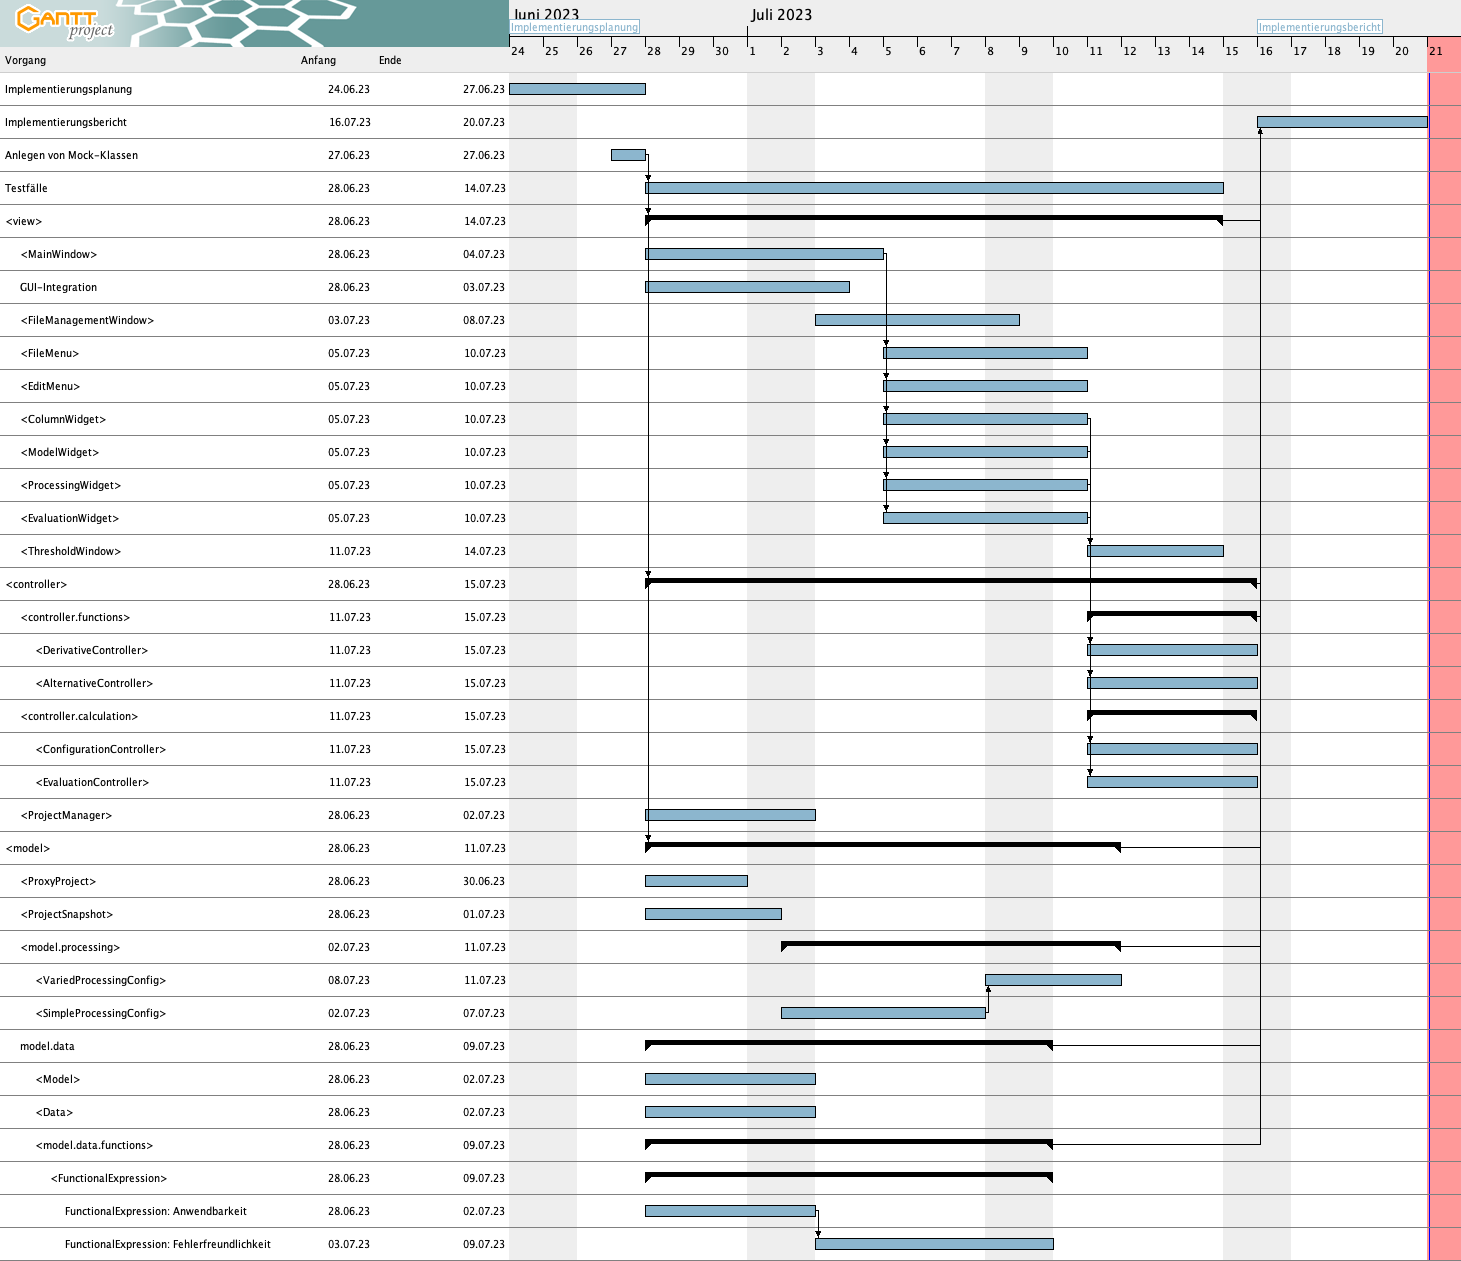
\includegraphics[width=12cm]{img/gantt_plan1.png}
    \label{fig:gantt_plan1}
    \caption{Zeitplan zu Beginn der Implementierungsphase.}
\end{figure}

Die Idee hinter dem Konzept war, die Pakete \emph{Model} und \emph{View} so früh wie möglich abzuschließen, da dort die zwei zeitkritischsten Aufgabenketten zu finden waren. In diesen Paketen gab es zusätzlich die Schwierigkeit, mit den externen Paketen \emph{\gls{biogeme}} und \emph{\gls{PyQt}} umgehen zu müssen. So sollte möglichst früh ein unabhängiges Testen beider Pakete ermöglicht werden. Beim \emph{Model}-Paket durch \emph{Unit-Testfälle}. Im \emph{View}-Paket hingegen durch Ausführen bzw. Darstellen der Benutzeroberfläche.

\subsection{Abweichungen und Verzögerungen}
%Welche Verzögerungen gab es im Implementierungsplan? Kann beispielsweise als zweites GANTT Diagramm am Ende dargestellt werden.

Nun soll die tatsächliche Umsetzung des ursprünglichen Plans (Abbildung~\ref{fig:gantt_plan1}) erläutert werden. Die nachfolgende Abbildung~\ref{fig:gantt_real} stellt diesen tatsächlichen Ablauf dar.

\begin{figure}[H]%
    \centering
    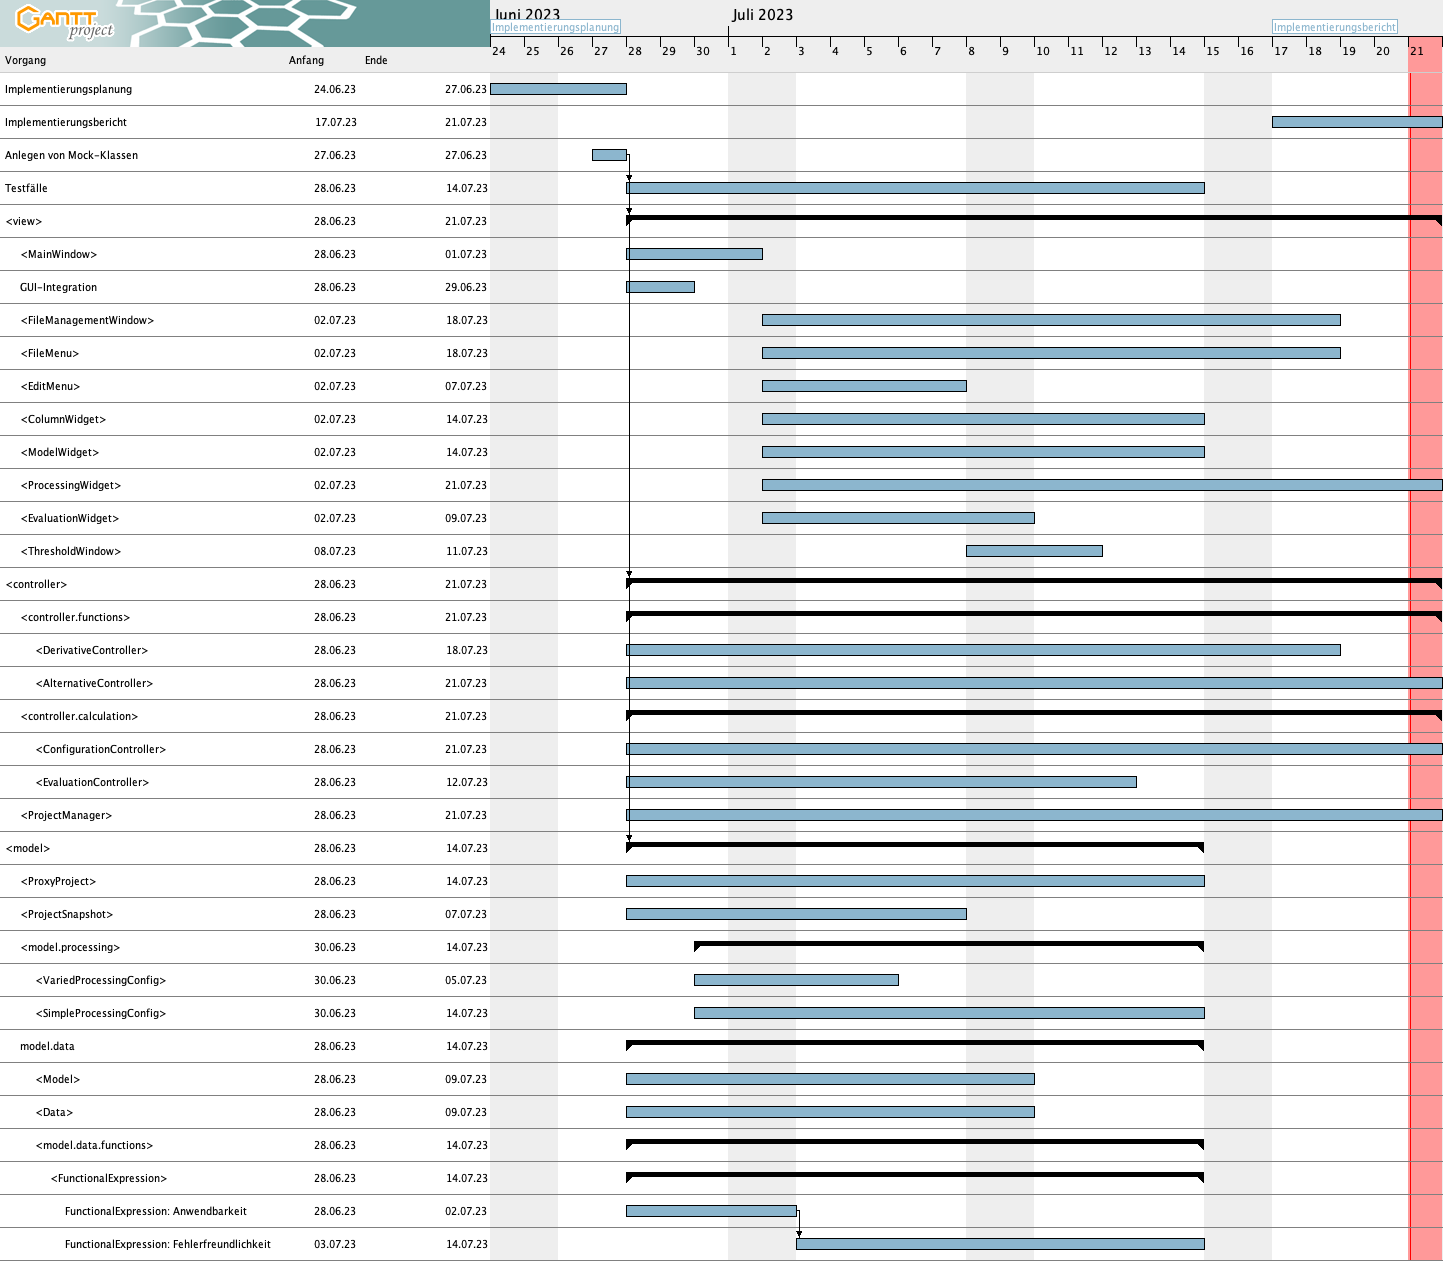
\includegraphics[width=12cm]{img/gantt_real.png}
    \label{fig:gantt_real}
    \caption{Tatsächlicher Ablauf der Implementierungsphase.}
\end{figure}

Durch Vergleichen von \ref{fig:gantt_plan1} und \ref{fig:gantt_real} können die Abweichungen festgestellt werden. So wurden die Aufgaben weniger, wie geplant, in einem kleinen Zeitfenster fertiggestellt, sondern eher kontinuierlich über die komplette Implementierungsphase verteilt umgesetzt.\\

Zu Beginn der Implementierungsphase gab es quasi keine Verzögerungen. Schneller als geplant verlief hier die Einbettung der Benutzeroberfläche, die zuvor mit einem GUI-Builder erstellt wurde. Hier wurde im Plan eine ganze Woche vorgesehen um unvorhersehbare Probleme mit \gls{PyQt} zu berücksichtigen. Unerwarteterweise gelang dies bereits nach zwei Tagen ohne echte Probleme.\\

In der zweiten Woche konnten leider nicht mehr alle Aufgaben termingerecht besprochen werden. Dies ist aus Sicht der Gruppe hauptsächlich darauf zurückzuführen, dass zu Beginn Unklarheiten darüber bestanden, was denn konkret zu implementieren war. Ebenfalls eine Rolle spielte sicherlich auch wenig Erfahrung mit Implementierungen.
Dieser Verzögerungstrend verstärkte sich leider in der dritten Woche nochmals.\\

Durch die Rückstände allgemein konnte die Anwendung leider erst in der letzten Woche aus der Benutzerperspektive vollständig getestet werden. Entsprechend wenig Zeit blieb für die Fehlerbehebung übrig.\\

\newpage
\section{Testübersicht}
%Übersicht zu Unittests und welches Framework

Für die Unittests wurde das Framework \texttt{unittest} aus der Python Standard Library verwendet. Da viele Funktionen der Software leicht und unabhängig voneinander getestet werden können, bietet das Modul ausreichende Funktionalität.

\subsection{View}
Für die grafische Benutzeroberfläche ist es nicht möglich automatisch ablaufende Tests zu schreiben. Demnach erfolgt hier das Testen manuell. \\
Zudem können hier einige Testfälle in die Phase der Qualitätssicherung verlegt werden.

\subsection{Controller}
Für die Controller wurden keine Testfälle erstellt. \\
Die Rolle des Controllers ist die Vermittelung zwischen Model und View. Somit ist auch die Programmlogik und Interaktion zwischen Klassen im Controller überschaubarer als die in den anderen beiden Paketen. Eine Einrichtung für Testfälle hatte hier also als keine hohe Priorität.

\subsection{Model}
\subsubsection{Data}
Im Bereich der Datenhaltung sind die FunctionalExpressions - also die Nutzenfunktionen und Attributsableitungen - der einzige Programmteil, der ausgiebig testbar ist. Hier müssen Überprüfungen des vom Nutzer übergebenen Ausdrucks erfolgen. Da sie möglichst umfangreich Fehler erkennen sollen, um diese dem Nutzer für Korrekturen zu übermitteln, ist die Anzahl an möglichen Testfällen enorm groß. Hier ist es wichtig, die Randfälle der validen und invaliden Ausdrücke zu kontrollieren. \\
Die Tests können in folgende Kategorien aufgeteilt werden:
\begin{itemize}
    \item Valide und invalide Syntax
        \begin{itemize}
            \item (Un)bekannte Ausdrücke
            \item Klammersetzung
        \end{itemize}
    \item Mathematische und logische Ausdrücke
        \begin{itemize}
            \item Grundrechenarten
            \item Vergleiche
            \item Potenzen
        \end{itemize}
    \item Legale Python Terme
        \begin{itemize}
            \item Built-In Funktionen auf der Whitelist
        \end{itemize}
    \item Illegale Python Terme
        \begin{itemize}
            \item Built-In Funktionen nicht auf der Whitelist
            \item Imports
            \item Schleifen
        \end{itemize}
    \item Neu definierte Datentypen
        \begin{itemize}
            \item Intervall
            \item GroupMap
        \end{itemize}
    \item Variablen
        \begin{itemize}
            \item Fehlende oder invalide Variablen
            \item Zyklische Abhängigkeiten
        \end{itemize}
\end{itemize}


\subsubsection{Processing}
Für das Testen des Berechnungsprozesses wurde eine Testklasse angelegt, welche die Berechnung eines Projektes mit einem Beispieldatensatz in \texttt{biogeme} durchführt. Damit kann die Berechnung auf Ordnungsmäßigkeit getestet werden.\\
Der Datensatz in der Testklasse wurde entnommen aus:\\ \url{https://github.com/michelbierlaire/biogeme/blob/master/examples/swissmetro/b01logit.py} (06.07.2023) \\


\newpage
\section{Statistiken}

Im Folgenden wird die Implementierungsphase durch verschiedene Statistiken quantifiziert. Dabei wird besonders auf zeitliche Verläufe, sowie Teamarbeit eingegangen.

\subsection{Verlauf}

Während der Implementierungsphase war die Arbeit am Projekt recht konstant. Nach dem ersten großen Comit am 28. Juni, bei dem die UI sowie die Klassengerüste erstellt. Dies hat viele Zeilen an Code auf einen Schlag hinzugefügt, daher das deutliche Maximum zum Beginn des Projektes, vgl Abb. \ref{fig:code_per_day}.

\begin{figure}[H]%
    \centering
    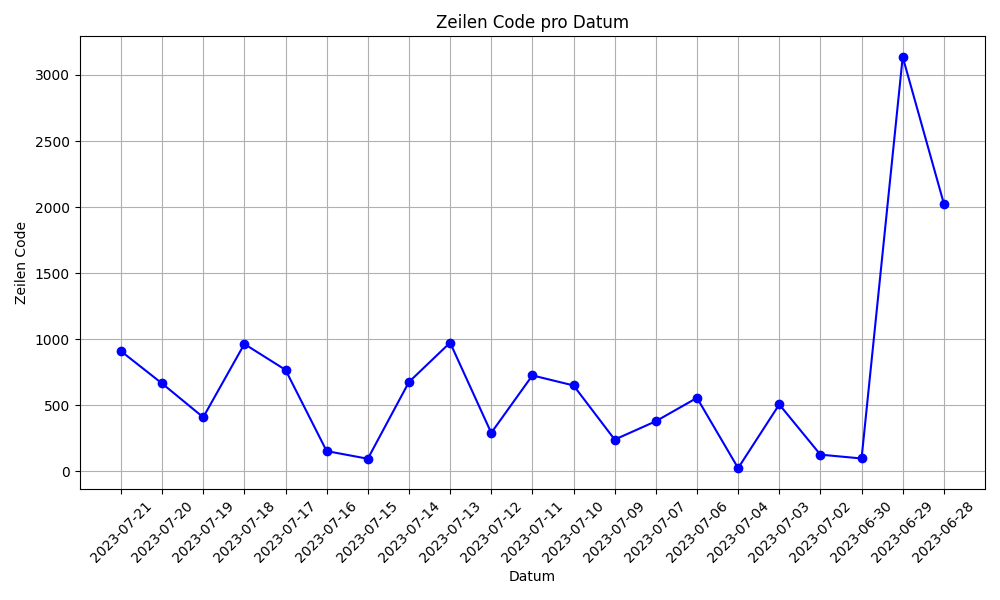
\includegraphics[width=12cm]{docs/implementation/report/img/CodeProTag.png}
    \label{fig:code_per_day}
    \caption{Zeilen Code Pro Tag.}
\end{figure}

Darauf war die Arbeit recht konstant, mit leichten natürlichen Schwankungen. Zur Mitte der Implementierungsphase, um den 14. Juli herum vgl. Abb. \ref{fig:code_per_day}, steigt die Produktivität leicht an, da die Klassenskelette ihre erste Implementierung erhalten. In der letzten Woche wird hauptsächlich Code überarbeitet. Daher gibt es weniger Code Zunahmen, da ebenfalls einige Zeilen wieder gelöscht werden. 

In Abb. \ref{fig:code_per_day} wird die anzahl an hinzugefügten Zeilen gegen das Datum geplottet um diesen Verlauf zu veranschaulichen. Die Zeilen Code pro Tag sind in dem Graphen die hinzugefügten Zeilen minus die entfernten.

\subsection{Repository}

Am Ende der Implentierungsphase gab es exklisive der Merge Commits 412 Commits zu allen Branches. Es gab 22 Pull Requests, sowie 39 Issues. Während der Implementierungsphase wurden 47 Dateien an Python Code hinzugefügt und bearbeitet.

In den Commits gab es 12,638 Zeilen Code die hinzugefügt wurden, sowie 750 Löschungen von Code. Auffallend dabei ist, dass die Anzahl der Commits zunimmt, während die Zahl der tatsächlich hinzugefügten Zeilen an Code abnimmt, vgl \ref{fig:commits_last_week}. Dies ist vorallem dadurch zu erklären, dass die Commits mit zunehmender Anpassung an die Schnittstellen des Codes der Teammilglieder kleiner werden. Bei der Feinarbeit und Behebung von Fehlern wurde Wert darauf gelegt kleine Commits zu machen, um die Reversibilität dieser möglicherweise ausnutzen zu können.

\begin{figure}[H]%
    \centering
    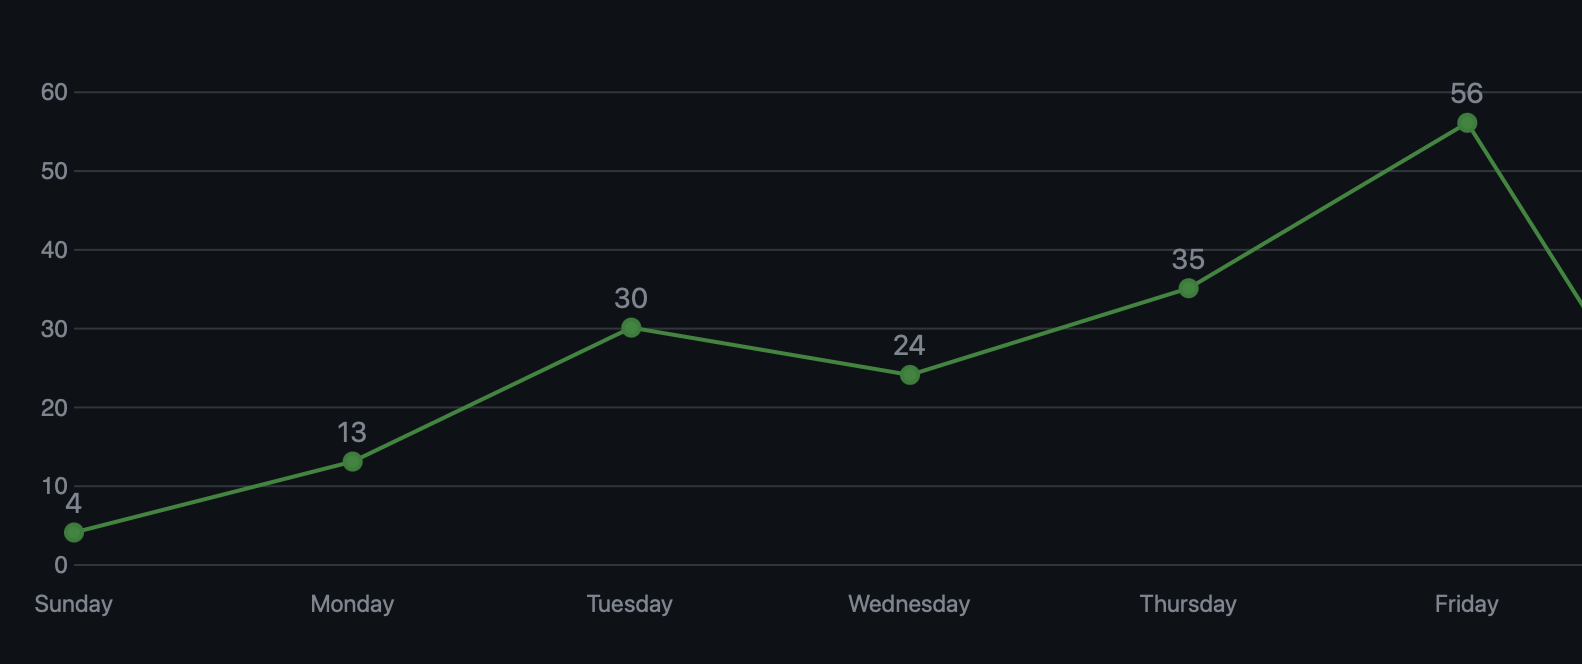
\includegraphics[width=12cm]{docs/implementation/report/img/CommitsDerLetztenWoche.png}
    \label{fig:commits_last_week}
    \caption{Anzahl Commits der letzten Woche der Implementierungsphase.}
\end{figure}

Am Ende der Implementierungsphase ergeben sich die absoluten Commits über alle Python Dateien in Tabelle \ref{tb: commits_overall}.

\begin{table}[]
\centering
\begin{tabular}{ll}
Autor            & Commits \\ \hline
Michael Schur    & 353     \\
Damian Reich     & 89      \\
Alissa Saleh     & 89      \\
Kevin Boehnke    & 45      \\
Floriane Bresser & 92     
\label{tb: commits_overall}
\end{tabular}
\caption{Commits}
\end{table}



\subsection{Teamwork}

Bei der Teamarbeit ist auffällig, dass Michael als Phasenverantwortlicher, sowie Maintainer des Repositories am meisten Zeilen Code geschrieben hat, nämlich 45 \%, vgl Abb.\ref{fig:teamwork}. Dies ist ebenso in der Committabelle (vgl. Abb. \ref{tb: commits_overall}) sichtbar.

\begin{figure}
\centering
\begin{tikzpicture}   
\pie[rotate=180]  
 {45/ Micheal Schur,  
     9/Damian Reich, 7/Kevin Boehnke, 22/Floriane Bresser, 17/Alissa Saleh}  
    
\end{tikzpicture} 
\caption{Codeverteilung} \label{fig:teamwork}
\end{figure}

Durch diesen Start zu Beginn der Implementierungsphase ergibt sich das Ungleichgewicht. Die anderen Personen haben durch die gleichmäßige Aufteilung an Klassen sowie Code in etwa gleichviel Code geschrieben. Diese Aussagen sind außerdem sehr ungenau, da hier das Codeformat eine große Rolle spielt. Personen, die viele Kommentare sowie lange Variablennamen verwenden, haben automatisch mehr Code, als kompakterer Codestil.
Die Zusammenarbeit erfolgte ansonsten ausgeglichen.

\clearpage
\printunsrtglossary
%\printglossary
\end{document}